\chapter{Le clavier}
Le but du clavier est de générer des tensions continues
différentes pour chaque note. Ces tensions continues
seront ensuite transformer en signal périodique par un
oscillateur contrôlé en tension (voir chapitre \ref{chap:vco}).

\section{Fonctionnement théorique}
Le principe de fonctionnement du clavier est assez simple.
Il peut être divisé en 3 blocs, comme représenté sur la
figure \ref{fig:keyboard-bloc}.

\begin{figure}[ht]
	\centering
	\includegraphics[scale=0.45]{img-keyboard/bloc.png}
	\caption{Schéma bloc du clavier.}
	\label{fig:keyboard-bloc}
\end{figure}

Le premier bloc permet le réglage des octaves, il couvre
les octaves 5 à 8. Il doit
être capable, à partir d'une tension constante d'approximativement
\unit{15}{\volt}, de fournir le plus précisément possible chacun 
des 4 niveaux de tensions indiqués sur la figure \ref{fig:keyboard-bloc}.
Ce premier bloc a donc un rôle de diviseur de tension.
Les niveaux de tensions inférieurs s'obtiennent des précédants en
les divisant successivement par deux, de la même manière
que la fréquence d'une note situé dans l'octave 5 correspond
à la moitié de lafréquence de cette même note dans l'octave 6.

A partir de ces niveaux de tensions, un deuxième bloc va
permettre le réglage des notes. Ce bloc divise sa tension d'entrée
de manière à faire correspondre à chaque note un niveau de tension
telle que \unit{1}{\milli\volt} corresponde à \unit{1}{\hertz}
\footnote{Et ce afin de répondre aux spécifications de l'oscillateur
contrôlé en tension, présenté au chapitre \ref{chap:vco}.}. Ce deuxième
bloc a donc à nouveau un rôle de diviseur de tension. Il est important
de noter que, lorsque aucune note n'est demandée, la tension de sortie
du deuxième bloc (et donc la tension de sortie du clavier) est égale à
sa tension d'entrée.

Enfin, le clavier est composé d'un troisième bloc. Ce dernier bloc permet
de corriger un défaut du clavier : sa sortie est non-nulle même si aucune
note n'est demandée et, par conséquent, le synthétiseur produit du son
même lorsque personne n’appuie sur une touche du clavier. Pour pallier
ce problème, le dernier bloc compare une fraction de la tension $E$ avec la
tension de sortie du clavier. Cette fraction, en l’occurrence 
$\frac{4}{5}$, a été choisie judicieusement afin de pouvoir détecter
si une touche est pressée ou non. Si $V_{\text{out}}$ est inférieur à
$\frac{4}{5}E$, alors une touche est pressée et le bloc ``Comparateur''
produira une tension continue de \unit{+15}{\volt}. Dans le cas contraire,
ce bloc produit une tension nulle. A partir de ces deux niveaux de tension,
un autre bloc situé situé à l'entrée de l'oscillateur contrôlé en tension ouvrira
son entrée si aucune touche n'est pressée, et la fermera dans le cas contraire, 
réglant ainsi le problème du son constant.
 
\section{Implémentation circuit et dimensionnement}
Comme indiqué dans la section précédente, le clavier
est constitué principalement de deux blocs de diviseurs
de tensions, comme le montre la figure \ref{fig:keyboard-circuit}.

\begin{figure}[ht]
	\centering
	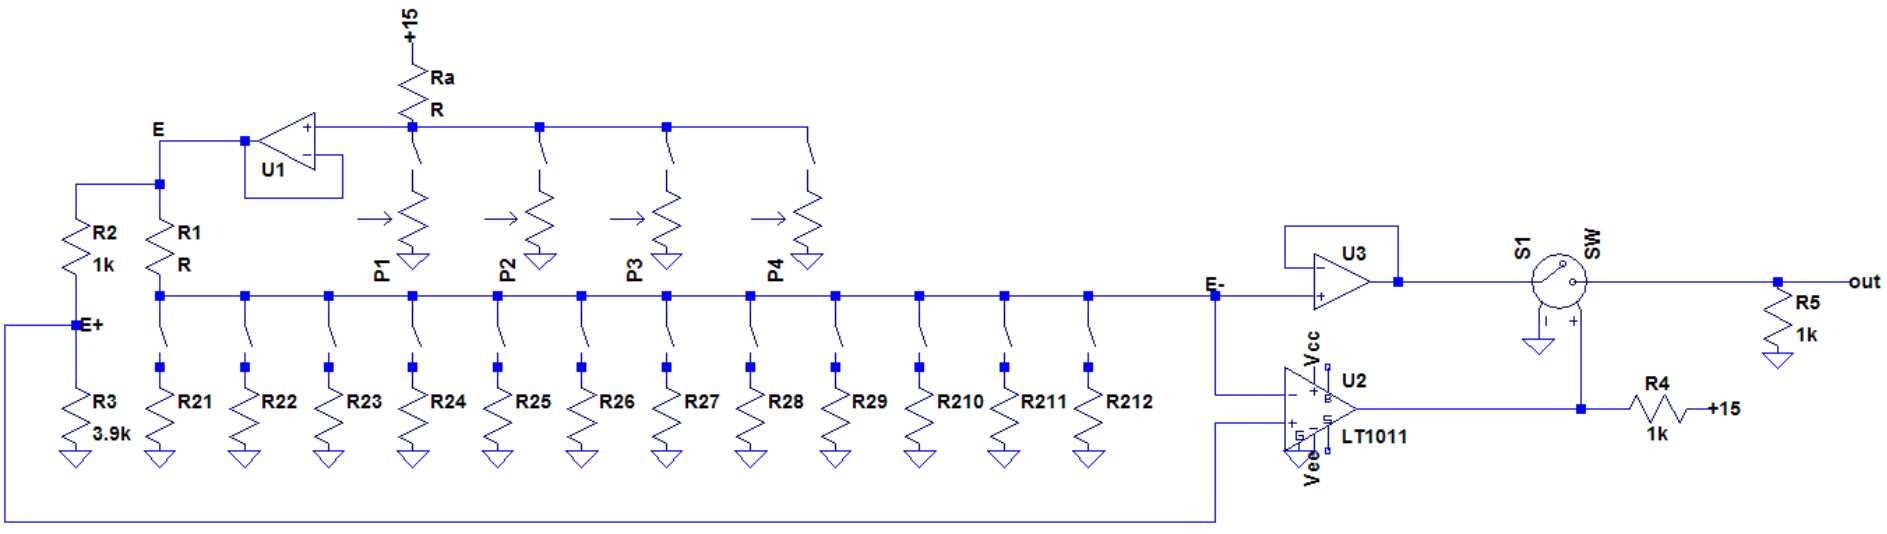
\includegraphics[scale=0.35]{img-keyboard/keyboard-circuit.png}
	\caption{Circuit du clavier. Dans un souci de lisibilité, les valeurs
	des résistances et des potentiomètres n'ont pas été indiquées sur ce
	schémas.}
	\label{fig:keyboard-circuit}
\end{figure}

Le premier réseau de diviseurs résistifs est constitué
de potentiomètres afin de permettre un calibrage des niveaux
de tensions $E$ (et donc de pallier les imprécisions de l'alimentation
\unit{+15}{\volt}). C'est en effet principalement ce paramètre qui
détermine la précision du clavier. Les interrupteurs constituant
ce premier réseau sont des interrupteurs à glissière.
Le tableau \ref{tab:dim-keyboard-first-bloc} résume
le dimensionnement de ce premier bloc.

\begin{table}[ht]
	\centering
	\begin{tabular}{|c|c|}
			\hline
				Résistance & Valeur (en\unit{}{\kilo\ohm}) \\
			\hline
				$R_a$ & 0.47 \\
			\hline
				$P_1$ (octave 8) & maximum 10 \\
			\hline
				$P_2$ (octave 7) & maximum 1 \\
			\hline
				$P_3$ (octave 6) & maximum 0.47 \\
			\hline
				$P_4$ (octave 5) & maximum 0.1 \\
			\hline
		\end{tabular}
	\caption{Résumé du dimensionnement du premier bloc.}
	\label{tab:dim-keyboard-first-bloc}
\end{table}

Le clavier des notes considéré ici comprend 12 touches, 
une pour chaque note et sa dièse correspondante. Les boutons
utilisés sont cette fois des boutons poussoirs.
Pour dimensionner ce bloc, il suffit d'appliquer la
formule suivante 

\[ \text{out} = E\frac{R_{2i}}{R_{2i} + R_1} \text{  avec  } i = 1\dots12. \]

Le dimensionnement complet du clavier se base
sur cette formule. En dimensionnant dans un premier
temps le clavier pour l'octave 8, l'obtention
de l'octave 7 est immédiate en divisant la tension
$E$ par deux, et ainsi de suite pour l'octave 6 et 5.

Le tableau \ref{tab:keyboard-dim} résume les résultats du dimensionnement
du clavier. Seules les valeurs standard de la série de Renard
E12 ont été utilisées. En utilisant une combinaison de 3
résistances en séries ou en parallèles, une erreur inférieure
à 0.01\% est garantie (sans tenir compte des tolérances des
résistances). En utilisant une combinaison plus économique
de seulement 2 résistances, des erreurs bien plus grandes
peuvent survenir (de l'ordre de 0.10\% à 0.30\%). Une telle
erreur est encore raisonnable pour l'oreille humaine qui ne
peut pas différencier deux sons dont la fréquence ne diffère
pas de plus de 0.6\%\cite{frequency-jnd}. Cependant, ces erreurs
risquent encore d'être amplifiées dans les blocs suivant du
synthétiseur, il est donc préférable de les minimiser au maximum
dans ce premier bloc.

\begin{table}[ht]
	\centering
		\begin{tabular}{|c|c|}
			\hline
				Résistance & Valeur (en\unit{}{\kilo\ohm}) \\
			\hline
				$R_1$ & 10 \\
			\hline
				$R_{21}$ (Do) & 2.7 + (1.8 | 12) \\
			\hline
				$R_{22}$ (Do\#) & 0.056 + (4.7 | 180) \\
			\hline
				$R_{23}$ (Ré) & 220 | (0.470 + 4.7) \\
			\hline
				$R_{24}$ (Ré\#) & 4.7 + (0.820 | 270) \\
			\hline
				$R_{25}$ (Mi) & 8.2 | 39 | 56 \\
			\hline
				$R_{26}$ (Fa) & 150 | (0.150 + 6.8)\\
			\hline
				$R_{27}$ (Fa\#) & 100 | 220 | 8.2 \\
			\hline
				$R_{28}$ (Sol) & 15 | 1000 | 18 \\
			\hline
				$R_{29}$ (Sol\#) & 22 | (0.330 + 15) \\
			\hline
				$R_{210}$ (La) & 10 + (0.120 | 2.7)\\
			\hline
				$R_{211}$ (La\#) & 3.3 + (680 | 8.2)\\
			\hline
				$R_{212}$ (Si) & 82 | (15 + 0.390)\\
			\hline
		\end{tabular}
	\caption{Résumé du dimensionnement du clavier.}
	\label{tab:keyboard-dim}
\end{table}

La présence d'un amplificateur suiveur entre le premier
réseau de diviseurs résistifs et le suivant est indispensable
pour les rendre indépendants.

Enfin, le comparateur et le switch présent sur la figure
\ref{fig:keyboard-circuit} fonctionne comme décrit dans la
section précédente.

\section{Confrontations théories et mesures}
Le tableau \ref{tab:keyboard-measure-vs-theory} donne quant
à lui les valeurs mesurées de la tension out. Les imprécisions
s'expliquent par les imprécisions des résistances et/ou du
calibrage.

\begin{table}[ht]
	\centering
		\begin{tabular}{|c|c|c|c|c|}
			\hline
				\specialcell{Octave $\rightarrow$ \\ Note $\downarrow$} & 5 & 6 & 7 & 8 \\
			\hline
				 Do & \unit{510}{\milli\volt} (-2.53\%) & \unit{1040}{\milli\volt} (-0.62\%) & \unit{2100}{\milli\volt} (+0.33\%) & \unit{4160}{\milli\volt} (-0.86\%) \\
			\hline
				 Do\# & \unit{547}{\milli\volt} (-1.26\%) & \unit{1100}{\milli\volt} (-0.78\%) & \unit{2230}{\milli\volt} (-0.58\%) & \unit{4460}{\milli\volt} (-0.565\%) \\
			\hline
				 Ré &  \unit{570}{\milli\volt} (-2.95\%) & \unit{1180}{\milli\volt} (+0.45\%) & \unit{2390}{\milli\volt} (+1.73\%) & \unit{4720}{\milli\volt} (+0.45\%) \\
			\hline
				 Ré\# & \unit{590}{\milli\volt} (-5.18\%) & \unit{1240}{\milli\volt} (-0.36\%) & \unit{2510}{\milli\volt} (+0.84\%) & \unit{4950}{\milli\volt} (-0.56\%) \\
			\hline
				 Mi & \unit{640}{\milli\volt} (-2.92\%) & \unit{1305}{\milli\volt} (-1.02\%) & \unit{2640}{\milli\volt} (+0.11\%) & \unit{5200}{\milli\volt} (-1.40\%) \\
			\hline
				 Fa & \unit{680}{\milli\volt} (-2.64\%) & \unit{1390}{\milli\volt} (-0.49\%) & \unit{2790}{\milli\volt} (-0.14\%) & \unit{5500}{\milli\volt} (-1.56\%) \\
			\hline
				 Fa\# & \unit{720}{\milli\volt} (-2.70\%) & \unit{1470}{\milli\volt} (-0.67\%) & \unit{2950}{\milli\volt} (-0.34\%) & \unit{5840}{\milli\volt} (-1.35\%) \\
			\hline
				 Sol & \unit{770}{\milli\volt} (-1.78\%) & \unit{1560}{\milli\volt} (-0.51\%) & \unit{3140}{\milli\volt} (+0.13\%) & \unit{6180}{\milli\volt} (-1.46\%) \\
			\hline
				 Sol\# & \unit{830}{\milli\volt} (-0.07\%)& \unit{1660}{\milli\volt} (-0.07\%) & \unit{3350}{\milli\volt} (+0.8\%) & \unit{6600}{\milli\volt} (-0.6\%) \\
			\hline
				 La & \unit{860}{\milli\volt} (-2.27\%) & \unit{1750}{\milli\volt} (-0.57\%) & \unit{3510}{\milli\volt} (-0.28\%) & \unit{6940}{\milli\volt} (-1.42\%) \\
			\hline
				 La\# & \unit{915}{\milli\volt} (-1.86\%) & \unit{1850}{\milli\volt} (-0.79\%) & \unit{3730}{\milli\volt} (+0.02\%) & \unit{7380}{\milli\volt} (-1.05\%) \\
			\hline
				 Si & \unit{970}{\milli\volt} (-1.79\%) & \unit{1960}{\milli\volt} (-0.78\%) & \unit{3960}{\milli\volt} (+0.22\%) & \unit{7790}{\milli\volt} (-1.42\%) \\
			\hline
		\end{tabular}
	\caption{Résumé des mesures effectués avec erreur relative calculées par comparaison avec
	le tableau suivant \url{http://fr.wikipedia.org/wiki/Note_de_musique}.}
	\label{tab:keyboard-measure-vs-theory}
\end{table}

Pour améliorer la précision du clavier, plusieurs pistes :
\begin{itemize}
	\item Utiliser des potentiomètres à la place des combinaisons
	de résistances, et calibrer le clavier avant chaque utilisation.
	Cependant cette solution n'est ni économique (un potentiomètre
	coûte beaucoup plus cher qu'une résistance) ni pratique (nécessitera
	un long calibrage) ;
	\item Utiliser des résistances plus précises ($\pm$ 1\% par exemple) ;
	\item Mesurer chaque résistance utilisée et remplacer celles dont la
	valeur est trop imprécise par une autre plus précise.
\end{itemize}